\documentclass[a4paper,11pt,final]{article}
        \usepackage{fancyvrb, color, graphicx, hyperref, ,amsmath, url}
        \usepackage{palatino}
        \usepackage[a4paper,text={16.5cm,25.2cm},centering]{geometry}

        \hypersetup
        {   pdfauthor = {Pweave},
            pdftitle={Published from BIOE232_HW20.py},
            colorlinks=TRUE,
            linkcolor=black,
            citecolor=blue,
            urlcolor=blue
        }
        \setlength{\parindent}{0pt}
        \setlength{\parskip}{1.2ex}
        
\makeatletter
\def\PY@reset{\let\PY@it=\relax \let\PY@bf=\relax%
    \let\PY@ul=\relax \let\PY@tc=\relax%
    \let\PY@bc=\relax \let\PY@ff=\relax}
\def\PY@tok#1{\csname PY@tok@#1\endcsname}
\def\PY@toks#1+{\ifx\relax#1\empty\else%
    \PY@tok{#1}\expandafter\PY@toks\fi}
\def\PY@do#1{\PY@bc{\PY@tc{\PY@ul{%
    \PY@it{\PY@bf{\PY@ff{#1}}}}}}}
\def\PY#1#2{\PY@reset\PY@toks#1+\relax+\PY@do{#2}}

\expandafter\def\csname PY@tok@gd\endcsname{\def\PY@tc##1{\textcolor[rgb]{0.63,0.00,0.00}{##1}}}
\expandafter\def\csname PY@tok@gu\endcsname{\let\PY@bf=\textbf\def\PY@tc##1{\textcolor[rgb]{0.50,0.00,0.50}{##1}}}
\expandafter\def\csname PY@tok@gt\endcsname{\def\PY@tc##1{\textcolor[rgb]{0.00,0.27,0.87}{##1}}}
\expandafter\def\csname PY@tok@gs\endcsname{\let\PY@bf=\textbf}
\expandafter\def\csname PY@tok@gr\endcsname{\def\PY@tc##1{\textcolor[rgb]{1.00,0.00,0.00}{##1}}}
\expandafter\def\csname PY@tok@cm\endcsname{\let\PY@it=\textit\def\PY@tc##1{\textcolor[rgb]{0.25,0.50,0.50}{##1}}}
\expandafter\def\csname PY@tok@vg\endcsname{\def\PY@tc##1{\textcolor[rgb]{0.10,0.09,0.49}{##1}}}
\expandafter\def\csname PY@tok@m\endcsname{\def\PY@tc##1{\textcolor[rgb]{0.40,0.40,0.40}{##1}}}
\expandafter\def\csname PY@tok@mh\endcsname{\def\PY@tc##1{\textcolor[rgb]{0.40,0.40,0.40}{##1}}}
\expandafter\def\csname PY@tok@go\endcsname{\def\PY@tc##1{\textcolor[rgb]{0.53,0.53,0.53}{##1}}}
\expandafter\def\csname PY@tok@ge\endcsname{\let\PY@it=\textit}
\expandafter\def\csname PY@tok@vc\endcsname{\def\PY@tc##1{\textcolor[rgb]{0.10,0.09,0.49}{##1}}}
\expandafter\def\csname PY@tok@il\endcsname{\def\PY@tc##1{\textcolor[rgb]{0.40,0.40,0.40}{##1}}}
\expandafter\def\csname PY@tok@cs\endcsname{\let\PY@it=\textit\def\PY@tc##1{\textcolor[rgb]{0.25,0.50,0.50}{##1}}}
\expandafter\def\csname PY@tok@cp\endcsname{\def\PY@tc##1{\textcolor[rgb]{0.74,0.48,0.00}{##1}}}
\expandafter\def\csname PY@tok@gi\endcsname{\def\PY@tc##1{\textcolor[rgb]{0.00,0.63,0.00}{##1}}}
\expandafter\def\csname PY@tok@gh\endcsname{\let\PY@bf=\textbf\def\PY@tc##1{\textcolor[rgb]{0.00,0.00,0.50}{##1}}}
\expandafter\def\csname PY@tok@ni\endcsname{\let\PY@bf=\textbf\def\PY@tc##1{\textcolor[rgb]{0.60,0.60,0.60}{##1}}}
\expandafter\def\csname PY@tok@nl\endcsname{\def\PY@tc##1{\textcolor[rgb]{0.63,0.63,0.00}{##1}}}
\expandafter\def\csname PY@tok@nn\endcsname{\let\PY@bf=\textbf\def\PY@tc##1{\textcolor[rgb]{0.00,0.00,1.00}{##1}}}
\expandafter\def\csname PY@tok@no\endcsname{\def\PY@tc##1{\textcolor[rgb]{0.53,0.00,0.00}{##1}}}
\expandafter\def\csname PY@tok@na\endcsname{\def\PY@tc##1{\textcolor[rgb]{0.49,0.56,0.16}{##1}}}
\expandafter\def\csname PY@tok@nb\endcsname{\def\PY@tc##1{\textcolor[rgb]{0.00,0.50,0.00}{##1}}}
\expandafter\def\csname PY@tok@nc\endcsname{\let\PY@bf=\textbf\def\PY@tc##1{\textcolor[rgb]{0.00,0.00,1.00}{##1}}}
\expandafter\def\csname PY@tok@nd\endcsname{\def\PY@tc##1{\textcolor[rgb]{0.67,0.13,1.00}{##1}}}
\expandafter\def\csname PY@tok@ne\endcsname{\let\PY@bf=\textbf\def\PY@tc##1{\textcolor[rgb]{0.82,0.25,0.23}{##1}}}
\expandafter\def\csname PY@tok@nf\endcsname{\def\PY@tc##1{\textcolor[rgb]{0.00,0.00,1.00}{##1}}}
\expandafter\def\csname PY@tok@si\endcsname{\let\PY@bf=\textbf\def\PY@tc##1{\textcolor[rgb]{0.73,0.40,0.53}{##1}}}
\expandafter\def\csname PY@tok@s2\endcsname{\def\PY@tc##1{\textcolor[rgb]{0.73,0.13,0.13}{##1}}}
\expandafter\def\csname PY@tok@vi\endcsname{\def\PY@tc##1{\textcolor[rgb]{0.10,0.09,0.49}{##1}}}
\expandafter\def\csname PY@tok@nt\endcsname{\let\PY@bf=\textbf\def\PY@tc##1{\textcolor[rgb]{0.00,0.50,0.00}{##1}}}
\expandafter\def\csname PY@tok@nv\endcsname{\def\PY@tc##1{\textcolor[rgb]{0.10,0.09,0.49}{##1}}}
\expandafter\def\csname PY@tok@s1\endcsname{\def\PY@tc##1{\textcolor[rgb]{0.73,0.13,0.13}{##1}}}
\expandafter\def\csname PY@tok@kd\endcsname{\let\PY@bf=\textbf\def\PY@tc##1{\textcolor[rgb]{0.00,0.50,0.00}{##1}}}
\expandafter\def\csname PY@tok@sh\endcsname{\def\PY@tc##1{\textcolor[rgb]{0.73,0.13,0.13}{##1}}}
\expandafter\def\csname PY@tok@sc\endcsname{\def\PY@tc##1{\textcolor[rgb]{0.73,0.13,0.13}{##1}}}
\expandafter\def\csname PY@tok@sx\endcsname{\def\PY@tc##1{\textcolor[rgb]{0.00,0.50,0.00}{##1}}}
\expandafter\def\csname PY@tok@bp\endcsname{\def\PY@tc##1{\textcolor[rgb]{0.00,0.50,0.00}{##1}}}
\expandafter\def\csname PY@tok@c1\endcsname{\let\PY@it=\textit\def\PY@tc##1{\textcolor[rgb]{0.25,0.50,0.50}{##1}}}
\expandafter\def\csname PY@tok@kc\endcsname{\let\PY@bf=\textbf\def\PY@tc##1{\textcolor[rgb]{0.00,0.50,0.00}{##1}}}
\expandafter\def\csname PY@tok@c\endcsname{\let\PY@it=\textit\def\PY@tc##1{\textcolor[rgb]{0.25,0.50,0.50}{##1}}}
\expandafter\def\csname PY@tok@mf\endcsname{\def\PY@tc##1{\textcolor[rgb]{0.40,0.40,0.40}{##1}}}
\expandafter\def\csname PY@tok@err\endcsname{\def\PY@bc##1{\setlength{\fboxsep}{0pt}\fcolorbox[rgb]{1.00,0.00,0.00}{1,1,1}{\strut ##1}}}
\expandafter\def\csname PY@tok@mb\endcsname{\def\PY@tc##1{\textcolor[rgb]{0.40,0.40,0.40}{##1}}}
\expandafter\def\csname PY@tok@ss\endcsname{\def\PY@tc##1{\textcolor[rgb]{0.10,0.09,0.49}{##1}}}
\expandafter\def\csname PY@tok@sr\endcsname{\def\PY@tc##1{\textcolor[rgb]{0.73,0.40,0.53}{##1}}}
\expandafter\def\csname PY@tok@mo\endcsname{\def\PY@tc##1{\textcolor[rgb]{0.40,0.40,0.40}{##1}}}
\expandafter\def\csname PY@tok@kn\endcsname{\let\PY@bf=\textbf\def\PY@tc##1{\textcolor[rgb]{0.00,0.50,0.00}{##1}}}
\expandafter\def\csname PY@tok@mi\endcsname{\def\PY@tc##1{\textcolor[rgb]{0.40,0.40,0.40}{##1}}}
\expandafter\def\csname PY@tok@gp\endcsname{\let\PY@bf=\textbf\def\PY@tc##1{\textcolor[rgb]{0.00,0.00,0.50}{##1}}}
\expandafter\def\csname PY@tok@o\endcsname{\def\PY@tc##1{\textcolor[rgb]{0.40,0.40,0.40}{##1}}}
\expandafter\def\csname PY@tok@kr\endcsname{\let\PY@bf=\textbf\def\PY@tc##1{\textcolor[rgb]{0.00,0.50,0.00}{##1}}}
\expandafter\def\csname PY@tok@s\endcsname{\def\PY@tc##1{\textcolor[rgb]{0.73,0.13,0.13}{##1}}}
\expandafter\def\csname PY@tok@kp\endcsname{\def\PY@tc##1{\textcolor[rgb]{0.00,0.50,0.00}{##1}}}
\expandafter\def\csname PY@tok@w\endcsname{\def\PY@tc##1{\textcolor[rgb]{0.73,0.73,0.73}{##1}}}
\expandafter\def\csname PY@tok@kt\endcsname{\def\PY@tc##1{\textcolor[rgb]{0.69,0.00,0.25}{##1}}}
\expandafter\def\csname PY@tok@ow\endcsname{\let\PY@bf=\textbf\def\PY@tc##1{\textcolor[rgb]{0.67,0.13,1.00}{##1}}}
\expandafter\def\csname PY@tok@sb\endcsname{\def\PY@tc##1{\textcolor[rgb]{0.73,0.13,0.13}{##1}}}
\expandafter\def\csname PY@tok@k\endcsname{\let\PY@bf=\textbf\def\PY@tc##1{\textcolor[rgb]{0.00,0.50,0.00}{##1}}}
\expandafter\def\csname PY@tok@se\endcsname{\let\PY@bf=\textbf\def\PY@tc##1{\textcolor[rgb]{0.73,0.40,0.13}{##1}}}
\expandafter\def\csname PY@tok@sd\endcsname{\let\PY@it=\textit\def\PY@tc##1{\textcolor[rgb]{0.73,0.13,0.13}{##1}}}

\def\PYZbs{\char`\\}
\def\PYZus{\char`\_}
\def\PYZob{\char`\{}
\def\PYZcb{\char`\}}
\def\PYZca{\char`\^}
\def\PYZam{\char`\&}
\def\PYZlt{\char`\<}
\def\PYZgt{\char`\>}
\def\PYZsh{\char`\#}
\def\PYZpc{\char`\%}
\def\PYZdl{\char`\$}
\def\PYZhy{\char`\-}
\def\PYZsq{\char`\'}
\def\PYZdq{\char`\"}
\def\PYZti{\char`\~}
% for compatibility with earlier versions
\def\PYZat{@}
\def\PYZlb{[}
\def\PYZrb{]}
\makeatother

        
\title{ HW20 - BIOE232}
\author{ Kyle King}
\date{ May 8, 2015}

\begin{document}
\maketitle
My Second Python Script!

\begin{Verbatim}[commandchars=\\\{\},frame=single,fontsize=\small, xleftmargin=0.5em]
\PY{c}{\PYZsh{} All the essentials}
\PY{k+kn}{import} \PY{n+nn}{numpy} \PY{k+kn}{as} \PY{n+nn}{np}  \PY{c}{\PYZsh{} np.\PYZus{}\PYZus{}version\PYZus{}\PYZus{}}
\PY{k+kn}{import} \PY{n+nn}{matplotlib.pyplot} \PY{k+kn}{as} \PY{n+nn}{plt}
\PY{k+kn}{import} \PY{n+nn}{csv}
\PY{k+kn}{from} \PY{n+nn}{decimal} \PY{k+kn}{import} \PY{o}{*}
\PY{k+kn}{from} \PY{n+nn}{pylab} \PY{k+kn}{import} \PY{o}{*}
\PY{n}{plt}\PY{o}{.}\PY{n}{close}\PY{p}{(}\PY{l+s}{\PYZdq{}}\PY{l+s}{all}\PY{l+s}{\PYZdq{}}\PY{p}{)}
\end{Verbatim}

Question 1

Assess how the dissociation constant (Kd) affects ligand binding to a
protein. Specifically, plot the fraction of a protein that is in the
bound state (CPL/PTotal) as a function of unbound ligand concentration
(CL) for three cases (a) Kd =10 mM; (b) Kd =1 mM; and (c) Kd = 0.1 mM.

\begin{Verbatim}[commandchars=\\\{\},frame=single,fontsize=\small, xleftmargin=0.5em]
\PY{c}{\PYZsh{} Declare varibales}
\PY{n}{R} \PY{o}{=} \PY{l+m+mf}{8.314}
\PY{n}{Kd} \PY{o}{=} \PY{p}{[}\PY{l+m+mi}{10}\PY{p}{,} \PY{l+m+mi}{1}\PY{p}{,} \PY{l+m+mf}{0.1}\PY{p}{]}  \PY{c}{\PYZsh{} mM}
\PY{n}{Cl} \PY{o}{=} \PY{n}{np}\PY{o}{.}\PY{n}{linspace}\PY{p}{(}\PY{l+m+mf}{0.001}\PY{p}{,} \PY{l+m+mi}{10}\PY{p}{,} \PY{n}{num}\PY{o}{=}\PY{l+m+mi}{1000}\PY{p}{)}  \PY{c}{\PYZsh{} ligand concentration from \PYZti{}0}
\PY{n}{to} \PY{l+m+mi}{10}\PY{n}{mM}
\PY{k}{for} \PY{n}{n} \PY{o+ow}{in} \PY{n}{Kd}\PY{p}{:}
    \PY{n}{ratio} \PY{o}{=} \PY{l+m+mi}{1}\PY{o}{/}\PY{p}{(}\PY{l+m+mi}{1}\PY{o}{+}\PY{p}{(}\PY{l+m+mi}{1}\PY{o}{/}\PY{p}{(}\PY{n}{n}\PY{o}{*}\PY{n}{Cl}\PY{p}{)}\PY{p}{)}\PY{p}{)}  \PY{c}{\PYZsh{} equation from lecture 19}
    \PY{c}{\PYZsh{} Plot function}
    \PY{n}{plot}\PY{p}{(}\PY{n}{Cl}\PY{p}{,} \PY{n}{ratio}\PY{p}{)}
\PY{n}{title}\PY{p}{(}\PY{l+s}{\PYZsq{}}\PY{l+s}{HW20: Q1 The ratio of CPL/PTotal}\PY{l+s}{\PYZsq{}}\PY{p}{)}
\PY{n}{xlabel}\PY{p}{(}\PY{l+s}{\PYZsq{}}\PY{l+s}{Cl}\PY{l+s}{\PYZsq{}}\PY{p}{)}
\PY{n}{ylabel}\PY{p}{(}\PY{l+s}{\PYZsq{}}\PY{l+s}{Ratio of CPL/PTotal}\PY{l+s}{\PYZsq{}}\PY{p}{)}
\PY{n}{legend}\PY{p}{(}\PY{n}{Kd}\PY{p}{)}
\PY{n}{grid}\PY{p}{(}\PY{n+nb+bp}{True}\PY{p}{)}
\PY{c}{\PYZsh{} show()}
\end{Verbatim}
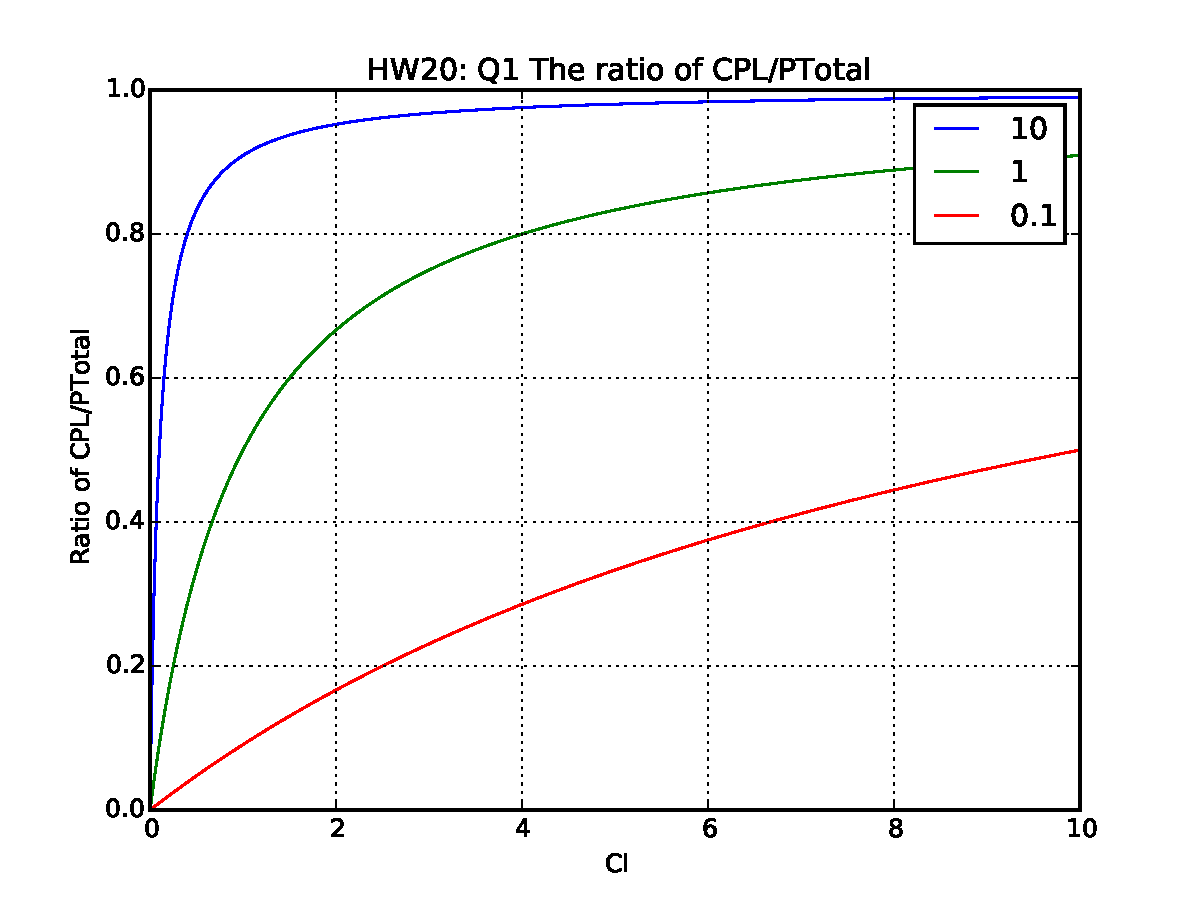
\includegraphics[width= \linewidth]{figures/BIOE232_HW20_figure3_1.pdf}

Question 2

Studies with the enzyme tyrosyl-tRNA synthetase indicate that the enzyme
can selectively bind the tyrosine moiety relative to the phenylalanine
moiety by a factor of 10\^{}5 at 300 K. What is the difference in
binding free energy and what types of interactions could be responsible
for such a difference?

\begin{Verbatim}[commandchars=\\\{\},frame=single,fontsize=\small, xleftmargin=0.5em]
\PY{n}{KaFactor} \PY{o}{=} \PY{n+nb}{pow}\PY{p}{(}\PY{l+m+mi}{10}\PY{p}{,} \PY{l+m+mi}{5}\PY{p}{)}
\PY{n}{deldelG} \PY{o}{=} \PY{o}{\PYZhy{}}\PY{n}{R}\PY{o}{*}\PY{l+m+mi}{300}\PY{o}{*}\PY{n}{log}\PY{p}{(}\PY{n}{KaFactor}\PY{p}{)}\PY{o}{/}\PY{l+m+mi}{1000}  \PY{c}{\PYZsh{} kJ/mole}
\PY{k}{print}\PY{p}{(}\PY{l+s}{\PYZdq{}}\PY{l+s}{The difference in binding free energy is }\PY{l+s+si}{\PYZpc{}d}\PY{l+s}{ kJ/mole}\PY{l+s}{\PYZdq{}} \PY{o}{\PYZpc{}} \PY{n}{deldelG}\PY{p}{)}
\PY{k}{print}\PY{p}{(}\PY{l+s}{\PYZdq{}}\PY{l+s}{This could be the result of a difference in one hydrogen bond}
\PY{p}{(}\PY{n}{about} \PY{l+m+mi}{5} \PY{o}{\PYZhy{}} \PY{l+m+mi}{30} \PY{n}{kJ}\PY{o}{/}\PY{n}{mole}\PY{p}{)}\PY{l+s}{\PYZdq{}}\PY{l+s}{)}
\end{Verbatim}
\begin{Verbatim}[commandchars=\\\{\},frame=leftline,fontsize=\small, xleftmargin=0.5em]
The difference in binding free energy is \PYZhy{}28 kJ/mole
This could be the result of a difference in one hydrogen bond (about 5
\PYZhy{} 30 kJ/mole)
\end{Verbatim}

Question 3

Several avidin-biotin binding systems have been studied (e.g., variant
proteins and ligands) at 300 K. The binding constant (Ka) and binding
enthalpy have been measured along with the force required to
mechanically unbind the protein-ligand complex (Fu). From the data
below, does the unbinding force correlate better with the free energy of
binding or the enthalpy of binding? (Moy et al. Sci. 266:257 (1994)).

\begin{Verbatim}[commandchars=\\\{\},frame=single,fontsize=\small, xleftmargin=0.5em]
\PY{k}{def} \PY{n+nf}{getNumericColumn}\PY{p}{(}\PY{n}{filename}\PY{p}{,} \PY{n}{column}\PY{p}{)}\PY{p}{:}
    \PY{n}{results} \PY{o}{=} \PY{n}{csv}\PY{o}{.}\PY{n}{reader}\PY{p}{(}\PY{n+nb}{open}\PY{p}{(}\PY{n}{filename}\PY{p}{)}\PY{p}{,} \PY{n}{delimiter}\PY{o}{=}\PY{l+s}{\PYZdq{}}\PY{l+s}{,}\PY{l+s}{\PYZdq{}}\PY{p}{,}
\PY{n}{quoting}\PY{o}{=}\PY{n}{csv}\PY{o}{.}\PY{n}{QUOTE\PYZus{}NONNUMERIC}\PY{p}{)}
    \PY{k}{return} \PY{p}{[}\PY{n}{result}\PY{p}{[}\PY{n}{column}\PY{p}{]} \PY{k}{for} \PY{n}{result} \PY{o+ow}{in} \PY{n}{results}\PY{p}{]}

\PY{c}{\PYZsh{} Import variables from csv file}
\PY{n}{filename} \PY{o}{=} \PY{l+s}{\PYZsq{}}\PY{l+s}{Q2data.csv}\PY{l+s}{\PYZsq{}}
\PY{c}{\PYZsh{} Convert to int for indexing}
\PY{n}{Count} \PY{o}{=} \PY{n}{np}\PY{o}{.}\PY{n}{array}\PY{p}{(}\PY{n+nb}{map}\PY{p}{(}\PY{n+nb}{int}\PY{p}{,} \PY{n}{getNumericColumn}\PY{p}{(}\PY{n}{filename}\PY{p}{,} \PY{l+m+mi}{0}\PY{p}{)}\PY{p}{)}\PY{p}{)}  \PY{c}{\PYZsh{} M\PYZca{}\PYZhy{}1}
\PY{n}{KaBase} \PY{o}{=} \PY{n}{getNumericColumn}\PY{p}{(}\PY{n}{filename}\PY{p}{,} \PY{l+m+mi}{1}\PY{p}{)}  \PY{c}{\PYZsh{} M\PYZca{}\PYZhy{}1}
\PY{n}{KaPow} \PY{o}{=} \PY{n}{getNumericColumn}\PY{p}{(}\PY{n}{filename}\PY{p}{,} \PY{l+m+mi}{2}\PY{p}{)}
\PY{n}{Fu} \PY{o}{=} \PY{n}{getNumericColumn}\PY{p}{(}\PY{n}{filename}\PY{p}{,} \PY{l+m+mi}{3}\PY{p}{)}  \PY{c}{\PYZsh{} pN}
\PY{n}{DelH} \PY{o}{=} \PY{n}{getNumericColumn}\PY{p}{(}\PY{n}{filename}\PY{p}{,} \PY{l+m+mi}{4}\PY{p}{)}  \PY{c}{\PYZsh{} Kcal/mol}

\PY{c}{\PYZsh{} Create Empty Array Ka}
\PY{n}{Ka} \PY{o}{=} \PY{p}{[}\PY{l+m+mi}{0}\PY{p}{]}\PY{o}{*}\PY{p}{(}\PY{n+nb}{len}\PY{p}{(}\PY{n}{Count}\PY{p}{)}\PY{p}{)}
\PY{c}{\PYZsh{} Fill array with values from csv file}
\PY{k}{for} \PY{n}{i} \PY{o+ow}{in} \PY{n}{Count}\PY{p}{:}
    \PY{n}{Ka}\PY{p}{[}\PY{n}{i}\PY{p}{]} \PY{o}{=} \PY{n}{KaBase}\PY{p}{[}\PY{n}{i}\PY{p}{]}\PY{o}{*}\PY{n+nb}{pow}\PY{p}{(}\PY{l+m+mi}{10}\PY{p}{,} \PY{n}{KaPow}\PY{p}{[}\PY{n}{i}\PY{p}{]}\PY{p}{)}
\PY{n}{DelG} \PY{o}{=} \PY{o}{\PYZhy{}}\PY{n}{R}\PY{o}{*}\PY{l+m+mi}{300}\PY{o}{*}\PY{n}{log}\PY{p}{(}\PY{n}{Ka}\PY{p}{)}\PY{o}{/}\PY{l+m+mi}{1000}  \PY{c}{\PYZsh{} kJ/mole}

\PY{n}{fig2} \PY{o}{=} \PY{n}{plt}\PY{o}{.}\PY{n}{figure}\PY{p}{(}\PY{p}{)}
\PY{n}{plt}\PY{o}{.}\PY{n}{scatter}\PY{p}{(}\PY{n}{DelG}\PY{p}{,} \PY{n}{Fu}\PY{p}{)}
\PY{n}{title}\PY{p}{(}\PY{l+s}{\PYZsq{}}\PY{l+s}{Free Energy versus Unbinding Force}\PY{l+s}{\PYZsq{}}\PY{p}{)}
\PY{n}{xlabel}\PY{p}{(}\PY{l+s}{\PYZsq{}}\PY{l+s}{Free Energy of Binding (kJ/mol)}\PY{l+s}{\PYZsq{}}\PY{p}{)}
\PY{n}{ylabel}\PY{p}{(}\PY{l+s}{\PYZsq{}}\PY{l+s}{Unbinding Force (Fu) in pN}\PY{l+s}{\PYZsq{}}\PY{p}{)}

\PY{n}{fig3} \PY{o}{=} \PY{n}{plt}\PY{o}{.}\PY{n}{figure}\PY{p}{(}\PY{p}{)}
\PY{n}{plt}\PY{o}{.}\PY{n}{scatter}\PY{p}{(}\PY{n}{DelH}\PY{p}{,} \PY{n}{Fu}\PY{p}{)}
\PY{n}{title}\PY{p}{(}\PY{l+s}{\PYZsq{}}\PY{l+s}{Binding Enthalpy versus Unbinding Force}\PY{l+s}{\PYZsq{}}\PY{p}{)}
\PY{n}{xlabel}\PY{p}{(}\PY{l+s}{\PYZsq{}}\PY{l+s}{Binding Enthalpy (kcal/mol)}\PY{l+s}{\PYZsq{}}\PY{p}{)}
\PY{n}{ylabel}\PY{p}{(}\PY{l+s}{\PYZsq{}}\PY{l+s}{Unbinding Force (Fu) in pN}\PY{l+s}{\PYZsq{}}\PY{p}{)}

\PY{c}{\PYZsh{} plt.show()}
\PY{k}{print}\PY{p}{(}\PY{l+s}{\PYZsq{}}\PY{l+s}{The Binding Enthalpy has a much stronger coorelation with Fu}\PY{l+s}{\PYZsq{}}\PY{p}{)}
\end{Verbatim}
\begin{Verbatim}[commandchars=\\\{\},frame=leftline,fontsize=\small, xleftmargin=0.5em]
The Binding Enthalpy has a much stronger coorelation with Fu
\end{Verbatim}
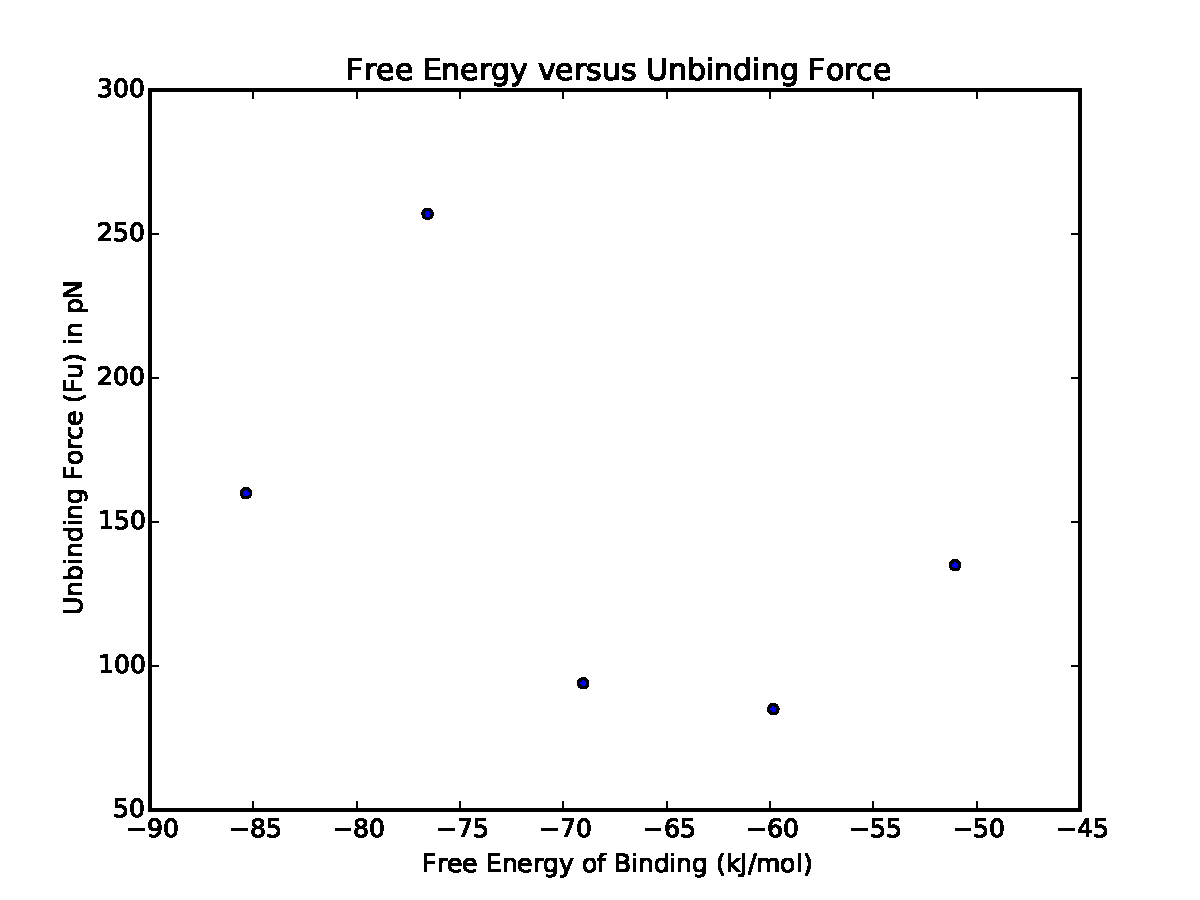
\includegraphics[width= \linewidth]{figures/BIOE232_HW20_figure5_1.pdf}
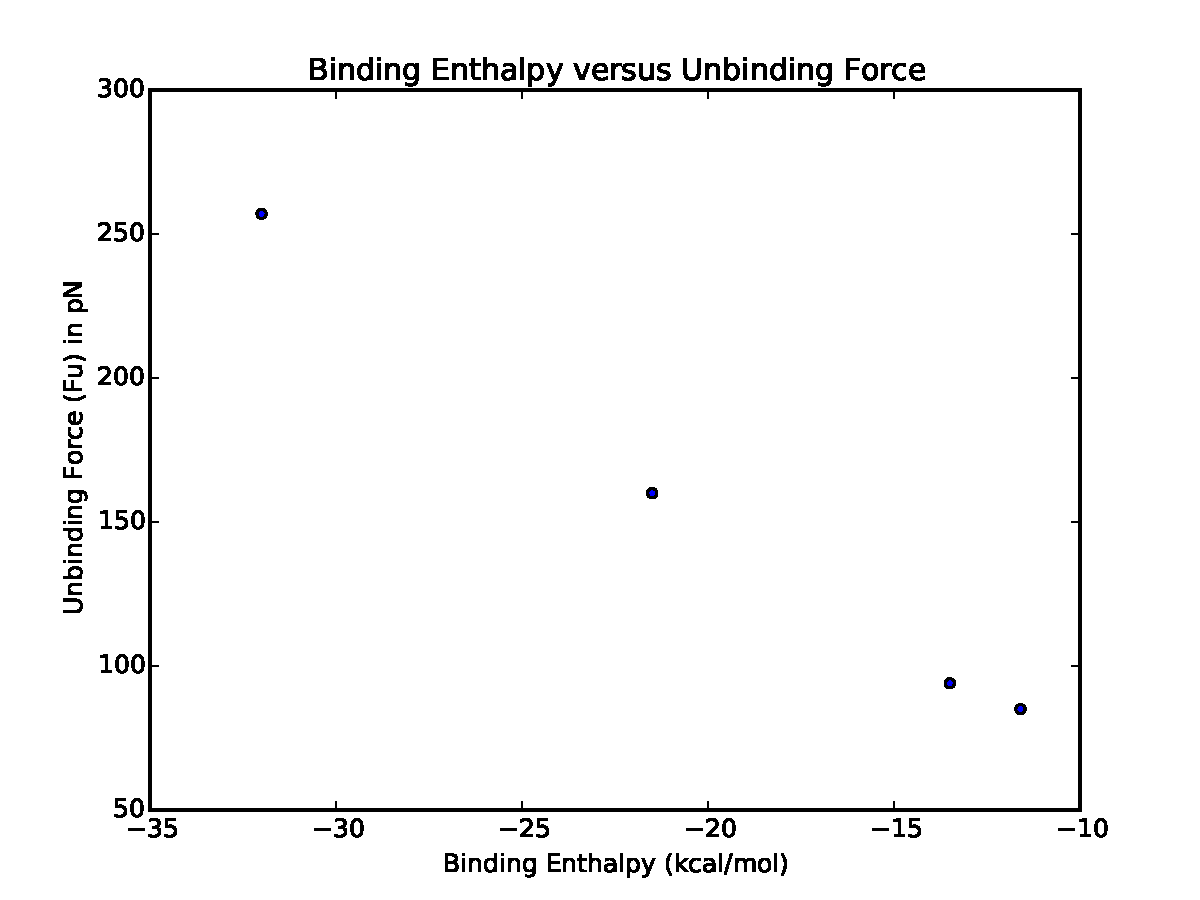
\includegraphics[width= \linewidth]{figures/BIOE232_HW20_figure5_2.pdf}

Question 4

See attached handwritten notes
\end{document}